A la hora de mantener una comunicación activa y evitar el control del brazo
por algún otro dispositivo se ha implementado el sistema de cifrado RSA tanto en el
\ac{SW} de \ac{S1} como en el de \ac{S2}.

Mediante el intercambio de mensajes en GCode un dispositivo externo puede autenticarse
contra la placa y esta verificarle, permitiendo seguir con las comunicaciones. Para
ello, se sigue el siguiente esquema:
\begin{itemize}
    \item Un dispositivo envía una orden \texttt{I1} al sistema \ac{S2}. Si dicho
    sistema no tiene todavía ningún dispositivo de confianza, acepta la orden \texttt{I1}.
    En otro caso, responderá con una orden \texttt{J10}.
    
    \item Si se acepta la orden \texttt{I1} entonces se procede a enviar el módulo
    `$n$' y la clave pública `$e$':
        \subitem El módulo se manda mediante una orden \texttt{I2 n}.
        \subitem La clave pública se manda mediante una orden \texttt{I3 e}.
    
    \item Además, se manda un mensaje aleatorio firmado con la clave privada `$d$'
    donde el otro dispositivo habrá de ``desfirmarla'' y volver a encriptarla, para
    mandarlo de vuelta al sistema \ac{S2}.
        \subitem El mensaje aleatorio firmado se manda con una orden \texttt{I4 msg}.
    
    \item El sistema \ac{S2} entonces queda a la espera de recibir el mensaje
    cifrado por el sistema \ac{S1}, donde lo desencriptará y comprobará el valor obtenido.
    Si el mensaje coincide, se acepta al nuevo dispositivo como de confianza y se podrán
    seguir con las comunicaciones. Se desactiva la orden I1.
        \subitem El mensaje cifrado ha de enviarse con un \texttt{I5 msg}, donde \ac{S2}
        responderá con la misma orden vacía.
\end{itemize}

En el siguiente diagrama (figura \ref{fig:rsa}) se pretende mostrar el comportamiento anterior:

\begin{figure}[H]
    \centering
    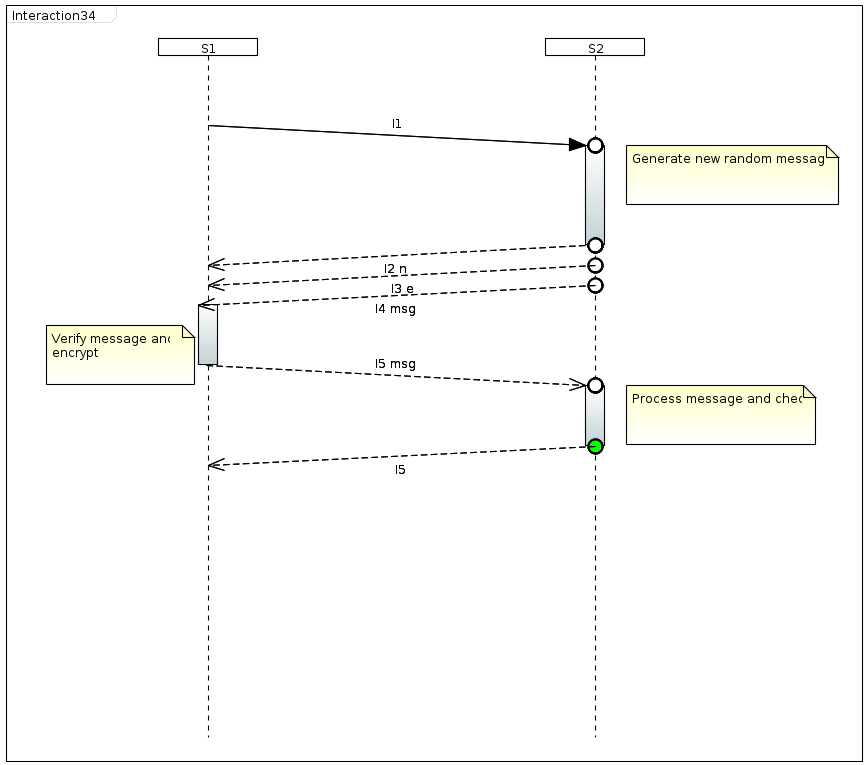
\includegraphics[width=.8\linewidth]{pictures/rsa.png}
    \caption{Diagrama de secuencia para el intercambio de las claves RSA.}
    \label{fig:rsa}
\end{figure}

Una vez se ha establecido la comunicación entre dispositivos es necesario mantenerla
activa, esto es, enviar mensajes periódicamente. Para ello se ha definido una función
de \textit{heartbeat} que mantiene dicha comunicación activa. Cada $\numprint[ms]{200}$
se espera un mensaje desde \ac{S1} del tipo \texttt{I7 msg}, con el mensaje aleatorio
intercambiado anteriormente cifrado. \ac{S2} lo verificará y si coincide con el mensaje
propio, actualiza el intervalo de tiempo.

Si se producen 5 fallos consecutivos (es decir, no hay mensajes válidos durante
un segundo) se deja de confiar en el dispositivo y es necesario voler a hacer
todo el proceso de intercambio de claves. Además, se generan nuevas claves RSA
por mayor seguridad.

Esta lógica está implementada en el fichero \texttt{main.c} (listado de código
\ref{lst:main_c}).
